% !TeX spellcheck = de_DE
% !TeX root = kristallographie_skript.tex

\subsubsection{Punktgruppen}

\begin{definition}[Punktgruppen]
Sei $G\leq\Isom(\IR^n)$ eine Gruppe von Bewegungen. Wenn es ein $x\in\IR^n$ gibt, das ein Fixpunkt von $G$ ist, d.h.
\[\forall g\in G: g(x)=x\]
dann nennt man $G$ eine \udot{Punktgruppe}. Ist zusätzlich auch $G\leq\Aut(\Lambda)$ erfüllt für einen Kristall $\Lambda\subseteq\IR^n$, dann nennt man $G$ eine \udot{kristallographische Punktgruppe}.
\end{definition}

\begin{lemma}[Punktgruppen vs. endliche Untergruppen]
Sei $G\leq\Isom(\IR^n)$ eine Gruppe von Bewegungen.
\begin{enumerate}
\item Ist $G$ endlich, dann ist $G$ eine Punktgruppe.
\item Ist $G$ kristallographisch, dann ist $G$ endlich.
\end{enumerate}
\end{lemma}
\begin{proof}
a. Wir haben das eigentlich schon einmal bewiesen: Wenn $x$ ein beliebiger Punkt und $G$ endlich ist, dann ist der Schwerpunkt der Basis
\[\frac{1}{\abs{G}} \sum_{g\in G} g(x)\]
ein Fixpunkt von ganz $G$.

\medbreak
b. Wir wählen uns ein Koordinatensystem so, dass der Nullpunkt ein Fixpunkt wird, sowie drei Punkte $a_1,a_2,a_3\in\Lambda$ im Kristall in drei unabhängige Richtungen von $0$ aus. Sei $r:=\max\Set{\norm{a_1},\norm{a_2},\norm{a_3}}$. Aufgrund der Mindestabstand-Bedingung für Kristalle ist
\[X:=\Set{a\in\Lambda | \norm{a}\leq r}\]
endlich. Ist $g\in\Aut(\Lambda)$ und $g(0)=0$, so sind die drei Punkte $g(a_1),g(a_2),g(a_3)$ wieder aus $X$. Weil $a_1,a_2,a_3$ linear unabhängig sind und $g$ als orthogonale Abbildung linear ist, ist $g$ eindeutig festgelegt durch diese drei Bildpunkte. Es gibt also maximal $\abs{X}^3$ viele Elemente von $G$.
\end{proof}

\begin{remark}
Nicht jede endliche Punktgruppe ist auch eine kristallographische Gruppe. Wir werden gleich z.B. sehen, dass die Ikosaedergruppe zwar endlich, aber nicht kristallographisch ist.
\end{remark}

\subsubsection{Kristallklassen und Gittersysteme}

\begin{remark}
Wir wissen, dass es nur eine sehr begrenzte Anzahl von (Konjugationsklassen von) endlichen Untergruppen von $O(\IR^3)$ gibt und wir haben eine Liste, die wir gut verstehen. In der Tat gibt es in jeder Dimension immer nur endlich viele endliche Untergruppen von $O(\IR^n)$.

Es bietet sich daher an, Kristalle danach zu klassifizieren, welche Punktgruppen sie haben. Naiv könnte man einfach die Punktgruppe $\Aut(\Lambda)_0$ betrachten, d.h. die Untergruppe aller derjenigen Symmetrien $g\in\Aut(\Lambda)$, die $g(0)=0$ erfüllen. Das Problem dabei ist, dass es außer der Identität überhaupt keine Symmetrien im Kristall geben muss, die den Nullpunkt festlassen. Der Nullpunkt könnte schlecht gewählt sein relativ zum Kristall, sodass er von keiner der möglichen, von $\id$ verschiedenen Drehung, keiner Spiegelung oder Drehinversion festgelassen wird (was ja die einzigen Bewegungen sind, die überhaupt Fixpunkte haben).

Und selbst wenn das nicht der Fall ist, könnte es sein, dass gar keine von $\id$ verschiedenen Drehungen, Spiegelungen oder Drehinversionen in $\Aut(\Lambda)$ existieren; jede Symmetrie könnte eine Translation, eine Schraubung oder Gleitspiegelung sein. Dann hätten wir keine Information gewonnen und würden viele sehr verschieden aussehende Kristalle in eine gemeinsame Kategorie \enquote{triviale Punktgruppe} einordnen.

Wenn wir das nicht wollen (und das wollen wir nicht), müssen wir uns überlegen, wie wir Symmetrien erfassen, die einen Translationsanteil $\neq 0$ haben, aber nicht gleich einer Translation sind, und wir den translationsfreien Anteil zweier solcher Symmetrien unterscheiden. Es stellt sich heraus, dass es eine andere, vom Kristall bestimmte Punktgruppe gibt, die das für uns tut.
\end{remark}

\begin{remark}
Wir erinnern uns, dass jede Bewegung $g:\IR^n\to\IR^n$ sich nach Wahl eines Nullpunkts schreiben lässt als Anwendung einer orthogonalen Bewegung $Q$ gefolgt von einer Translation $\tau_v$, d.h.
\[\forall x\in\IR^n: g(x)=Q(x)+v\]
\end{remark}

\begin{lemma}
Sei $\Lambda\subseteq\IR^n$ ein Kristall. Dann operiert $G=\Aut(\Lambda)$ auf der Translationsuntergruppe bzw. dem Translationsgitter $Trans(\Lambda)$ durch Konjugation:
\[{^g \tau_w} := g\circ\tau_w\circ g^{-1} \quad\text{bzw.}\quad {^g w} = Q(w)\]
wobei wie eben $g(x)=Q(x)+v$ ist.
\end{lemma}
\begin{proof}
Zunächst müssen wir beweisen, dass ${^g \tau_w}=g\circ\tau_w\circ g^{-1}$ wieder eine Translation ist.

Was für eine Bewegung ist das? Es gilt für alle Punkte $x\in\IR^n$:
\begin{align*}
(g\circ\tau_w\circ g^{-1})(x) &= g(\tau_w(g^{-1}(x))) \\
&= Q(\tau_w(Q^{-1}(x-v))+v \\
&= Q(Q^{-1}(x-v)+w)+v \\
&= Q(Q^{-1}(x-v))+Q(w)+v &\text{da $Q$ linear ist}\\
&= x-v+Q(w)+v &\text{da }Q\circ Q^{-1}=\id\\
&= x+Q(w) \\
&=\tau_{Q(w)}(x)
\end{align*}
D.h. $g\circ\tau_w\circ g^{-1} = \tau_{Q(w)}$ ist wieder eine Translation.

\medbreak
Nun müssen wir nachweisen, dass dies wirklich eine Operation ist. Es gilt
\[1\circ\tau_w\circ 1^{-1} = \tau_w\circ 1 = \tau_w\]
also ${^1 w} = w$ und
\[g\circ(h\circ\tau_w\circ h^{-1})\circ g^{-1} = (g\circ h)\circ\tau_w\circ(h^{-1}\circ g^{-1}) = (g\circ h)\circ\tau_w\circ(g\circ h)^{-1}\]
also ${^g(^h w)} = {^{g\circ h}w}$. Das sind genau die Bedingungen, die wir brauchen.
\end{proof}

\begin{remark}
Man beachte, dass bzgl. dieser Operation die Translationen und nur die Translationen trivial operieren, d.h. von jedem $g\in G$ ist nur der translationsfreie Anteil (das $Q$) relevant.

Das vereinfacht die Art der vorkommenden Symmetrien drastisch: Wenn $g\in\Aut(\Lambda)$ eine Schraubung um Winkel $\alpha$ ist, dann ist die Symmetrie $R_g:w\mapsto{^g w}$ des Translationsgitters nur noch eine Drehung um Winkel $\alpha$. Analog ist $R_s$ eine Spiegelung, wenn $s$ eine (Gleit)spiegelungen war.
\end{remark}

\begin{corollary}
Sei $\Lambda\subseteq\IR^n$ ein Kristall. Die Gruppe $\Set{R_g | g\in G}$ ist eine kristallographische Punktgruppe. Insbesondere ist sie endlich.
\end{corollary}
\begin{proof}
Alle $R_g$ sind orthogonal. Insbesondere fixieren sie alle den Nullvektor. Also ist es eine Punktgruppe. Sie ist eine Untergruppe von $\Aut(Trans(\Lambda))$, also eine kristallographische Punktgruppe. 
\end{proof}

\begin{remark}
Sofern die Übungsaufgaben zu Normalteilern und Quotienten bearbeitet wurden: Die Translationsuntergruppe $\mathcal{T}\leq\Aut(\Lambda)$ ist ein Normalteiler (da -- wie eben bewiesen -- konjugieren mit beliebigen $g\in G$ aus Translationen wieder Translationen macht). Es ist also wohldefiniert, von der Quotientengruppe $\Aut(\Lambda) / \mathcal{T}$ zu sprechen.

Die Punktgruppe $\Set{R_g | g\in G}$ ist kanonisch isomorph zu diesem Quotienten, indem wir $R_g$ und $g\mathcal{T}$ identifizieren.
\end{remark}

\begin{definition}[Kristallklassen]
Wir sagen, dass zwei Kristalle $\Lambda,\Lambda'\subseteq\IR^n$ in derselben \udot{Kristallklasse} sind, wenn die beiden Punktgruppen
\[\Set{R_g | g\in\Aut(\Lambda)} \leq \Aut(Trans(\Lambda))_0 \]
und
\[\Set{R_g | g\in\Aut(\Lambda')} \leq \Aut(Trans(\Lambda'))_0 \]
in $O(\IR^n)$ konjugiert sind.
\end{definition}

\begin{remark}[Geometrische Interpretation -- Operation auf dem 3-Torus]
Wir wählen uns eine elementare Basiszelle $Z$ des Kristalls $\Lambda$. Eine Möglichkeit, die Punktgruppe $\Set{R_g | g\in G}=\Aut(\Lambda)/\mathcal{T}$ geometrisch zu interpretieren ist folgende:

Wenn wir in $Z$ die obere mit der unteren, die rechte mit der linken und die vordere mit der hinteren Seitenfläche verkleben, erhalten wir einen sogenannten 3-Torus $T$. Man stelle sich das wie gewisse, simple Computerspiele (z.B. Snake) vor: Wenn man am rechten Rand hinausläuft, kommt man sofort am linken Rand wieder hinein ins \enquote{Spielfeld} usw. (Im Gegensatz zur Veranschaulichung des 2-Torus als Donuts / Schwimmreifens / Kaffeetasse / ... ist diese Konstruktion des 2- bzw. 3-Torus jedoch ohne Krümmung, weil wir abstandserhaltend arbeiten wollen)

\medbreak
$g\in\Aut(\Lambda)$ kann nun auch aufgefasst werden als eine Symmetrie $S_g: T\to T$, nämlich die folgende: Für einen Input-Punkt $x\in T$ ist $S_g(x)$ derjenige Punkt, der wie folgt entsteht:
\begin{enumerate}
\item Zunächst fassen wir $x\in T$ als Punkt $\hat{x}\in Z$ auf.
\item Dann wenden wir $g$ auf diesen Punkt an.
\item Das Ergebnis $g(\hat{x})$ liegt in irgendeiner Zelle $Z'$, die eine translatierte Kopie $Z'=\tau(Z)$ der Basiszelle ist (möglicherweise mit einer Verschiebung um $0$, d.h. $\tau=\id$). Wir machen die Translation $\tau$ rückgängig und erhalten wieder einen Punkt in $\hat{y}=\tau^{-1}(g(\hat{x}))\in Z$.
\item Diesen fassen wir wieder als Punkt $y\in T$ im 3-Torus auf. Das ist dann unser Output-Punkt: $y=:S_g(x)$.
\end{enumerate}

Man beachte, dass diese Symmetrien $S_g: T\to T$ nicht analog zu den Symmetrien $R_g: Trans(\Lambda)\to Trans(\Lambda)$ sein müssen. Insbesondere haben sie noch nicht die Eigenschaft, die wir haben wollen, dass translatorische Anteile ignoriert werden. Ist etwa $g$ eine Schraubung oder eine Drehung, so ist $R_g: Trans(\Lambda) \to Trans(\Lambda)$ in beiden Fällen eine Drehung. Hingegen operieren Schraubungen und Drehungen nicht unbedingt identisch auf dem 3-Torus.

Dies ist also ein weiteres Beispiel dafür, dass dieselbe Gruppe nicht nur auf eine Weise als Symmetriegruppe auftreten kann. Dieselbe Gruppe (hier $\Aut(\Lambda) /\mathcal{T}$) kann auf verschiedenen Objekten (hier etwa: Dem Translationsgitter und dem 3-Torus) auf völlig verschiedene Arten operieren.

\medbreak
Was bedeutet das für uns? Das heißt, dass wir unser Ziel, Translationsanteile vollkommen zu ignorieren, noch nicht erreicht haben mit dieser Konstruktion. Nach Konstruktion wirken zwar alle Translationen $\tau_w$ mit $w\in Trans(\Lambda)$ trivial auf $T$, aber Schraubungen und Gleitspiegelungen können Translationsanteile enthalten, die selber nicht in $Trans(\Lambda)$ liegen. Das ist etwa der Grund, wieso wir in $T$ immer noch einen Unterschied zwischen Drehungen und Schraubungen sehen können.

Ein Ausweg daraus liefert folgende Beobachtung: Das Motiv $M$ definiert uns eine \emph{endliche} Punktmenge in $T$, die die Eigenschaft
\[\forall g\in\Aut(\Lambda): S_g(M) = M\]
hat. Wir können $\set{S_g | g\in\Aut(\Lambda)}$ also mit einer Untergruppe der Permutationsgruppe $\Sym(M)$ identifizieren. Insbesondere handelt es sich also um eine \emph{endliche} Gruppe.

Ist $n$ die Ordnung dieser Gruppe, so schlussfolgern wir aus dem Satz von Lagrange, dass die Elementordnung $ord(S_g)$ stets ein Teiler von $n$ sein muss. Insbesondere gilt also $S_{g^n} = S_g^n = \id_T$.

Die einzigen Symmetrien des Kristalls, die auf dem Torus wie die Identität wirken, sind aber die Translationen. Es muss mit anderen Worten einen Translationsvektor $w\in Trans(\Lambda)$ geben, sodass $g^n = \tau_w$ ist. Wenn nun $g$ eine Schraubung oder Gleitspiegelung mit Verschiebungsvektor $v$ ist, dann ist $g(x)=Q(x)+v$ und $Q(v)=v$. Somit ist
\[\forall x: x+w=\tau_w(x)=g^n(x) = Q^n(x)+nv\]
Wir folgern $w=nv$, d.h. $v=\frac{1}{n}w\in \frac{1}{n}Trans(\Lambda)$.

In Worten: Die vorkommenden Verschiebungsvektoren sind nicht beliebig: Es muss sich genau um das $\frac{1}{n}$-fache eines Gittervektors handeln.

\medbreak
Was bedeutet das geometrisch? Wenn wir nicht die Basiszelle $Z$, sondern die parallele Zelle $\tilde{Z}:=\frac{1}{n}Z$ mit gleichem Basispunkt, gleichen Kantenrichtungen, aber $\frac{1}{n}$-fachen Kantenlängen (und somit Volumen $\frac{1}{n}^3\cdot\operatorname{vol}(Z)$) betrachten, dann haben wir einen 3-Torus $\tilde{T}$ (mit kleinerem Volumen!) gefunden, der nun folgende Eigenschaft hat: Genauso wie alle Translationen mit Verschiebungsvektor $w\in Trans(\Lambda)$ trivial auf $T$ operieren, operieren nun auch alle Translationen mit Verschiebungsvektor $v\in\frac{1}{n}Trans(\Lambda)$ trivial auf $\tilde{T}$.

Insbesondere bedeutet das, dass von $g(x)=Q(x)+v$ nur der $Q$-Anteil übrig bleibt, weil $v\in\frac{1}{n}Trans(\Lambda)$ ist. Damit haben wir nun endlich (nach deutlich mehr Aufwand) auch in dieser geometrischen Sichtweise den gleichen Effekt erzielt wie zuvor: Die Symmetrien $\tilde{S}_g: \tilde{T}\to\tilde{T}$ unterscheiden nicht mehr zwischen Drehungen und Schraubungen, Spiegelungen und Gleitspiegelungen etc.
\end{remark}

\begin{remark}
Es gibt immer endlich viele, aber möglicherweise sehr viele Kristallklassen in einer Dimension. Im dreidimensionalen Raum gibt es z.B. 32 Kristallklassen. Und trotzdem sehen Kristalle in verschiedene Kristallklassen manchmal sehr ähnlich aus.

Deshalb möchten wir zusätzlich zur Einteilung in Kristallklassen die Kristalle etwas gröber einteilen und zwar nach der Form der möglichen Basiszellen des Kristalls.
\end{remark}

\begin{definition}[Gittersysteme]
Es seien $\Lambda, \Lambda' \subseteq\IR^n$ zwei Kristalle. Dazu gehören zwei Translationsgitter $T:=Trans(\Lambda)$ und $T':=Trans(\Lambda')$.

Wir sagen $\Lambda,\Lambda'$ sind im selben \udot{Gittersystem}, wenn die Punktgruppen $\Aut(T)_0$ und $\Aut(T')_0$ in $O(\IR^n)$ konjugiert sind.
\end{definition}

\begin{remark}
Man beachte, dass nach Konstruktion $\set{R_g | g\in \Aut(\Lambda)} \leq \Aut(T)_0$ ist, aber es muss keine Gleichheit bestehen, d.h. es könnte Symmetrien des Translationsgitters geben, die nicht Symmetrien des Kristalls sind. Der Grund ist, dass wir hierbei das Motiv der Kristalle vergessen. Nicht jedes Element von $\Aut(T)_0$ muss das Motiv stabilisieren.
\end{remark}

\subsubsection{Klassifikation der dreidimensionalen Gittersysteme}

\begin{remark}
Unser Ziel ist es jetzt, die dreidimensionalen Gittersysteme zu klassifizieren. Laut Definition müssen wir also die Punktgruppen aller Translationsgitter bestimmen. Konkret wollen wir in diesem Abschnitt den folgenden Satz beweisen:
\end{remark}

\begin{theoremdef}[Klassifikation der dreidimensionalen Gittersysteme]
Betrachte ein Translationsgitter $T=\IZ v_1+\IZ v_2+\IZ v_3\subseteq\IR^3$. Es sei $G:=\Aut(T)_0$ die Punktgruppe des Nullpunkts.

$G$ ist dann genau eine der folgenden sieben Gruppen: $G$ ist erzeugt von ...
\begin{enumerate}
\item \udot{Triklin}: ... der Inversion.

\item \udot{Monoklin}: ... der Inversion und einer 2-zähligen Drehung.

Jeder monokline Kristall besitzt eine Basiszelle, in denen eine Basisrichtung eine zweizählige Symmetrieachse ist (d.h. der Kristall hat eine \SI{180}{\degree}-Drehung, -Drehinversion oder -Schraubung um diese Achse) und die anderen beiden Basisrichtungen senkrecht auf ihr stehen.

\item \udot{Orthorhombisch}: ... der Inversion und zwei 2-zähligen Drehungen um zueinander senkrechte Achsen.

Jeder orthorhombische Kristall besitzt eine Basiszelle mit drei rechten Winkeln, in der alle drei Basisrichtungen zweizählige Symmetrieachsen sind.

\item \udot{Trigonal}: ... der Inversion, einer 2- und einer 3-zähligen Drehung um zueinander senkrechte Achsen.

Jeder trigonale Kristall besitzt eine Basiszelle, in der die Winkel $\SI{90}{\degree}$, $\SI{90}{\degree}$ und $\SI{120}{\degree}$ sind, eine Basisrichtung eine dreizählige Symmetriachse ist und die anderen beiden zweizählige Symmetrieachsen.

\item \udot{Tetragonal}: ... der Inversion, einer 2- und einer 4-zähligen Drehung um zueinander senkrechte Achsen.

Jeder tetragonale Kristall besitzt eine Basiszelle mit drei rechten Winkeln, in der eine Basisrichtung eine vierzählige und die anderen beiden zweizählige Symmetrieachsen sind.

\item \udot{Hexagonal}: ... der Inversion, einer 2- und einer 6-zähligen Drehung um zueinander senkrechte Achsen.

Jeder hexagonal Kristall besitzt eine Basiszelle, in der die Winkel $\SI{90}{\degree}$, $\SI{90}{\degree}$ und $\SI{120}{\degree}$ sind, eine Basisrichtung eine sechszählige Symmetriachse ist und die anderen beiden zweizählige Symmetrieachsen.

\item \udot{Kubisch}: ... der Inversion, einer 3- und einer 4-zähligen Drehung (alternativ: zwei 4-zähligen Drehungen um zueinander senkrechte Achsen).

Jeder kubische Kristall besitzt eine würfelförmige Basiszelle, in der durch alle drei Basisrichtungen vierzählige Symmetrieachsen laufen und durch alle vier Raumdiagonalen jeweils dreizählige Symmetrieachsen.
\end{enumerate}
Diese Gruppen sind ineinander enthalten wie in Diagramm \ref{kristalle:hasse_diagramm_Gittersysteme} angegeben.
\end{theoremdef}

\begin{figure}[ht]
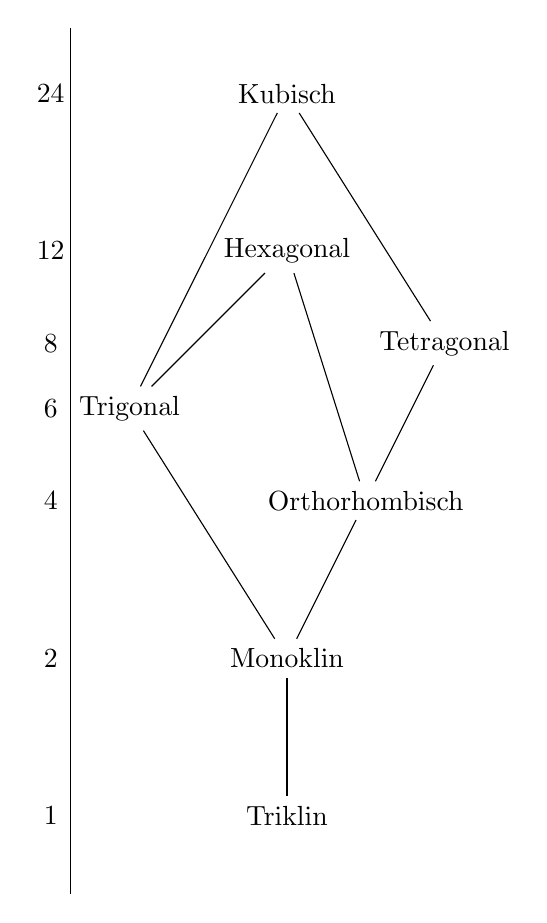
\begin{tikzpicture}[yscale=2]
\node (kubisch) at (0,4.585) % ~\log_2(24) = \log_2(6)+2
	{Kubisch};
\node at (-3,4.585) {24};
\node (hexagonal) at (0,3.585) % ~\log_2(12) = \log_2(6)+1
	{Hexagonal};
\node at (-3,3.585) {12};
\node (tetragonal) at (2,3)
	{Tetragonal};
\node at (-3,3) {8};
\node (trigonal) at (-2,2.585) % ~\log_2(6)
	{Trigonal};
\node at (-3,2.585) {6};
\node (orthorhombisch) at (1,2)
	{Orthorhombisch};
\node at (-3,2) {4};
\node (monoklin) at (0,1)
	{Monoklin};
\node at (-3,1) {2};
\node (triklin) at (0,0)
	{Triklin};
\node at (-3,0) {1};

\draw (-2.75,-0.5) -- (-2.75,5); 

\path
(triklin) edge (monoklin)
(monoklin) edge (orthorhombisch)
(monoklin) edge (trigonal)
(orthorhombisch) edge (hexagonal)
(orthorhombisch) edge (tetragonal)
(tetragonal) edge (kubisch)
(trigonal) edge (kubisch)
(trigonal) edge (hexagonal);
\end{tikzpicture}
\caption{Hasse-Diagramm der sieben dreidimensionalen Gittersysteme zusammen mit der Ordnung der jeweiligen Drehgruppe}
\label{kristalle:hasse_diagramm_Gittersysteme}
\end{figure}

\begin{remark}
Wir kennen bereits diverse endliche Untergruppen von $O(\IR^3)$ aus \ref{gruppen:klassifikation_drehgruppen_in_3D}. Dies sind erstens nicht alle kristallographischen Punktgruppen und zweitens eine unendliche Liste von Gruppen. Das ist schon einmal schlecht, weil in dem obigen Satz ja nur sieben Gruppen vorkommen. Wir müssen uns also überlegen, wie wir zeigen, dass bis auf diese sieben keine anderen Gruppen als $\Aut(T)_0$ vorkommen kann.

Das werden wir in zwei Schritten tun: Mit Hilfe der sogenannten \enquote{kristallographischen Restriktion} werden wir von unendlich vielen auf elf Fälle reduzieren. Im zweiten Schritt werden wir mit einer genaueren Analyse von den übrigen elf noch einmal vier ausschließen.
\end{remark}

\begin{theorem}[Kristallographische Einschränkung]\label{kristalle:kristallographische_einschraenkung}
Sei $\Lambda\subseteq\IR^n$ ein Kristall und $g\in\Aut(\Lambda)$ eine Drehung oder Schraubung um den Winkel $\alpha$.
\begin{enumerate}
\item Die einzigen möglichen Winkel sind $\SI{180}{\degree}=\frac{2\pi}{2}, \SI{120}{\degree}= \frac{2\pi}{3}, \SI{90}{\degree}=\frac{2\pi}{4}$, $\SI{60}{\degree}=\frac{2\pi}{6}$ oder $\alpha=0$.
\item Ist $\alpha\neq 0$, dann gibt es unabhängige Vektoren $v_1, v_2, v_3$ im Translationsgitter (nicht notwendigerweise eine Basis des Translationsgitters), sodass
\begin{enumerate}
\item $v_1$ in Richtung der Drehachse von $g$ zeigt und
\item $v_2$ und $v_3$ senkrecht auf $v_1$ stehen,
\end{enumerate}
Ist außerdem $\alpha\neq\pi$, dann können wir zusätzlich auch
\begin{enumerate}[resume]
\item $v_3={^g v_2}$
\end{enumerate}
erreichen.
\end{enumerate}
\end{theorem}

\begin{proof}
Wir betrachten die orthogonale Abbildung $R_g:=w\mapsto{^g w}$ auf dem Translationsgitter. In unserem Fall ist das eine Drehung.

Die Drehachse geht natürlich durch den Nullpunkt, aber weil wir mit Translationen verknüpfen können, hat das Translationsgitter natürlich auch Drehsymmetrien mit gleichem Winkel und paralleler Drehachse durch jeden anderen Punkt des Gitters.

Wir legen uns das Koordinatensystem so, dass die $z$-Achse in Richtung der Drehachse zeigt und betrachten einen beliebigen Vektor $v=\begin{psmallmatrix}x\\y\\z\end{psmallmatrix}$ im Translationsgitter, der nicht in Richtung der Drehachse zeigt, d.h. $(x,y)\neq(0,0)$. Solche Vektoren gibt es, z.B. müssen immer mindestens zwei Vektoren in jeder Gitterbasis diese Eigenschaft haben. O.B.d.A. können wir sogar annehmen, dass wir das Koordinatensystem so gewählt haben, dass $y=0$ ist.

\medbreak
Da $R$ das Translationsgitter auf sich selbst abbildet, sind $Rv$ und $R^{-1}v$ wieder Vektoren im Gitter. Wir können explizit beschreiben, was $Rv$ und $R^{-1}v$ sind:
\[Rv =\begin{pmatrix}\cos(\alpha)x\\\sin(\alpha)x\\z\end{pmatrix}, R^{-1}v =\begin{pmatrix}\cos(\alpha)x\\-\sin(\alpha)x\\z\end{pmatrix}\]
Daraus folgt, dass der Gittervektor $v_2:=Rv+R^{-1}v-2v$ die Form
\[(R+R^{-1})v-2v = \begin{pmatrix}(2\cos(\alpha)-2)x\\0\\0\end{pmatrix}\]
hat.

Kann dies der Nullvektor sein? Das geht nur, wenn $2\cos(\alpha)-2=0$, d.h. $\alpha=0$ ist. Ansonsten haben wir einen von Null verschiedenen Vektor $v_2$ im Gitter gefunden, der senkrecht zur Drehachse ist.

Wenn wir noch einen zweiten, Vektor $v'$ nehmen, der von $v$ und der Drehachse linear unabhängig ist (z.B. wieder einen Basisvektor), dann können wir auf dieselbe Weise einen von $v_2$ linear unabhängigen Vektor $v_3$ finden, der senkrecht zur Drehachse ist. Wenn $\alpha$ nicht zufällig $\pi$ ist, dann ist $Rv_2$ auch linear unabhängig von $v_2$ und senkrecht zur Drehachse.

\medbreak
Wir betrachten also zwei Gitterpunkte $A\neq B$ mit Differenzvektor $v_2$, die in einer  Ebene senkrecht zur Drehachse liegen (z.B. den Nullpunkt und $v_2$ selbst). Daraus können wir die Punkte $A'$ und $B'$, indem wir die Drehungen anwenden, deren Achsen durch $A$ bzw. $B$ laufen.

Rechnen:
\[B=A+v_2, \qquad B'=A+Rv_2\]
\[A=B-v_2, \qquad A'=B-R^{-1}v_2\]
Die Punkte $A'$,$B'$ sind selbst Gitterpunkte, d.h. ihre Differenz $B'-A'=(A-B)+Rv_2+R^{-1}v_2=(R+R^{-1}-1)v_2$ ist selbst wieder ein Vektor im Translationsgitter. Wir rechnen nach: Wenn $v_2=\begin{psmallmatrix}x_2\\0\\0\end{psmallmatrix}$ ist, dann ist
\[(R+R^{-1}-1)v_2 = \begin{pmatrix}(2\cos(\alpha)-1)x_2\\0\\0\end{pmatrix}\]
d.h. $(R+R^{-1})v_2-v_2$ ist ein Vielfaches von $v_2$. Da beides Gittervektoren sind, ist das nur möglich, wenn es sich um ein \emph{ganzzahliges} Vielfaches handelt, d.h. $2\cos(\alpha)-1$ muss eine ganze Zahl sein!

Die einzigen möglichen Werte für $\alpha\in[0,\pi]$, die das erfüllen, sind:
\[\begin{array}{c|ccccc}
\alpha & 0 & \frac{2\pi}{6} & \frac{2\pi}{4} & \frac{2\pi}{3} & \pi \\
\hline
\cos(\alpha) & 1 & \frac{1}{2} & 0 & -\frac{1}{2} & -1 \\
2\cos(\alpha)-1 & 1 & 0 & -1 & -2 & -3 \\
2\cos(\alpha)-2 & 0 & -1 & -2 & -3 & -4
\end{array}\]
Das zeigt schon einmal, dass nicht beliebige Winkelwerte für Drehungen eines Translationsgitters vorkommen können.

\medbreak
Kehren wir zurück zu $v=\begin{psmallmatrix}x\\0\\z\end{psmallmatrix}$ und $v_2=\begin{psmallmatrix}(2\cos(\alpha)-2)x\\0\\0\end{psmallmatrix}$. Aus der Tabelle mit den expliziten Werten lesen wir ab, dass für $k\in\set{1,2,3,4}$ der Gittervektor $v_1:=v_2+kv=\begin{psmallmatrix}0\\0\\kz\end{psmallmatrix}$ in Richtung der Drehachse liegt.
\end{proof}

\begin{remark}
Das schließt also insbesondere auch aus, dass es Kristalle mit Dodekaeder-Symmetrien gibt, denn ansonsten müsste es Drehungen der Ordnung 5 im Translationsgitter geben.

Mehr Einschränkungen gibt es jedoch nicht mehr, d.h. jede der endlichen Drehgruppen, die ausschließlich 2-, 3-, 4- oder 6-zählige Symmetrien hat, kommt tatsächlich in der Symmetriegruppe eines dreidimensionalen Kristalls vor.

Der hier vorgestellte Beweis verallgemeinert sich nicht auf höhere Dimensionen. Es gibt zwar in jeder Dimension nur eine endliche Liste von möglichen Elementordnungen, aber je höher die Dimension ist, desto höher kann die Ordnung der vorkommenden Drehungen/Schraubungen sein. Beispielsweise hat das $n$-dimensionale Würfelgitter $\IZ^n$ eine Symmetrie der Ordnung $n+1$. Insbesondere gibt es im $\IR^4$ schon Kristalle mit 5-zähligen Symmetrien.
\end{remark}

\begin{example}
\begin{enumerate}
\item Der Kristall $\IZ^3\subseteq\IR^3$ hat die Würfelgruppe in seiner Symmetriegruppe. Also besitzt er sowohl 3- als auch 4-zählige Drehsymmetrien. Wenn es eine 4-zählige Drehung gibt, gibt es auch eine 2-zählige.
\item Der Kristall $(\IZ+\IZ(\tfrac{1+\sqrt{3}i}{2})) \times \IZ \subseteq \IC\times\IR = \IR^3$ (Honigwaben) hat eine 6-zählige Drehsymmetrie.
\end{enumerate}
\end{example}

\begin{remark}
Wenn wir linear unabhängige Vektoren $v_1,v_2,v_3\in Trans(\Lambda)$ gefunden haben, z.B. mit Hilfe der obigen Konstruktion, dann ist $T_0:=\IZ v_1+\IZ v_2+\IZ v_3 \leq Trans(\Lambda)$ ein Untergitter, das ggf. weniger Gittervektoren enthält und eine größere Basiszelle hat. Die so konstruierte Basiszelle ist vielleicht größer als sie sein müsste (sie ist also keine \emph{elementare} Basiszelle), kann aber den Vorteil haben, geometrisch einfacher zu sein als eine elementare Basiszelle, z.B. ist in der Situation des obigen Satzes $v_2$ und $v_3$ senkrecht auf $v_1$, d.h. die Basiszelle mit den Kanten $v_1,v_2,v_3$ ist ein rechtwinkliges Prisma mit einem Parallelogramm als Grundfläche (das auch ein Rechteck oder ein Quadrat sein kann) Es muss keine Gitterbasis von $Trans(\Lambda)$ geben, die diese Eigenschaft besitzt.

Wenn wir diese Konstruktion jeweils auf diejenige Drehung mit der höchsten vorkommenden Ordnung anwenden, dann erhalten wir die Basiszellen aus dem Klassifikationssatz.
\end{remark}

\begin{proof}[Beweis der Klassifikation der Gittersysteme]
Es ist $G\leq O(\IR^3)$ und somit $D:=G\cap SO(\IR^3)$ eine Untergruppe von $G$, die Untergruppe aller \emph{orientierungserhaltenden} Symmetrien. Man beachte nun, dass die Inversion im Nullpunkt stets in $G$ enthalten ist, da dies immer eine Symmetrie von $T$ ist (es muss keine Symmetrie des $T$ zugrundeliegenden Kristalls sein).

Jedes Element $g\in G$ ist entweder bereits in $D$ enthalten oder $-g$ ist in $D$ enthalten. Daher ist $G=\Set{\pm g | g\in G} = \braket{-1,D}$. Es genügt also, die möglichen Drehgruppen zu klassifizieren. $G$ (und damit auch $D$) ist endlich, weil es eine kristallographische Punktgruppe ist. Wir kennen aufgrund von \ref{gruppen:klassifikation_drehgruppen_in_3D} alle möglichen, endlichen Drehgruppen und aufgrund von \ref{kristalle:kristallographische_einschraenkung} können aber nur solche Drehgruppen auftreten, in denen alle Drehungen Ordnung 1,2,3,4 oder 6 haben. Das reduziert unsere Liste der möglichen Gruppen drastisch von unendlich vielen zu nur noch elf:

$D$ könnte sein:
\begin{enumerate}
\item Zyklisch: $D$ wird von einer 1-, 2-, 3-, 4- oder 6-zähligen Drehung erzeugt.
\item Diedergruppe: $D$ wird von einer \SI{180}{\degree}-Drehung und einer 2-,3,-4, oder 6-zähligen Drehung mit senkrechter Drehachse erzeugt.
\item Tetraedergruppe: $D$ könnte die Drehgruppe eines Tetraeders sein.
\item Würfel-/Oktaedergruppe: $D$ könnte die Drehgruppe eines Würfels sein
\end{enumerate}

Die Gruppen, die wir uns als Ziel gesetzt haben, sind darin bereits enthalten: Es sind genau die triviale Gruppe (=triklin), die 2-zählige Drehung (=monoklin), die 2-, 3-, 4- bzw. 6-zähligen Diedergruppen (orthorhombisch, trigonal, tetragonal bzw. hexagonal) sowie die Würfelgruppe (=kubisch). Wir müssen noch ausschließen, dass zyklische Gruppen der Ordnungen 3,4,6 oder die Tetraedergruppe vorkommen. Ein Weg, das einzusehen, ist, die folgende Behauptung zu beweisen:

\medbreak
\fbox{\parbox{\textwidth}{Ist $g\in\Aut(T)_0$ eine 3-, 4- oder 6-zählige Drehung, dann besitzt $T$ eine Gitterbasis $w_1,w_2,w_3$, sodass $w_1$ parallel zu Drehachse von $g$ ist und $w_3=g(w_2)$ ist.}}

\medbreak
Dazu benutzen wir, dass es eine Gitterbasis $v_1,v_2,v_3$ gibt, in der $v_1$ parallel zur Drehachse ist. Indem wir ein Koordinatensystem so wählen, dass die $z$-Richtung genau entlang der Drehachse verläuft, haben die Vektoren also die folgenden Koordinaten
\[v_1 = \begin{pmatrix} 0 \\ 0 \\ z_1 \end{pmatrix}, v_2 = \begin{pmatrix} x_2 \\ y_2 \\ z_2 \end{pmatrix}, v_3 = \begin{pmatrix} x_3 \\ y_3 \\ z_3 \end{pmatrix}\]

Wenn wir nun alle Gittervektoren in die $x$-$y$-Ebene projizieren, erhalten wir ein zweidimensionales Gitter $T'$, mit Gitterbasis
\[v_2' := \begin{pmatrix} x_2 \\ y_2\end{pmatrix}, v_3' := \begin{pmatrix} x_3 \\ y_3 \end{pmatrix}.\]
Da das ursprüngliche Gitter die Rotation $g$ als Symmetrie hatte, hat auch das projizierte Gitter $g$ als Rotationssymmetrie. Wir wissen aus \ref{kristalle:gitterbasen_2D_kuerzeste_vektoren}, dass wir eine Gitterbasis dieses Gitters finden können, indem wir kürzeste Vektoren suchen. Sei $w_2'\in T'\setminus\set{0}$ ein kürzester Vektor. Dann ist $w_3':=g(w_2')\in T'$ ebenfalls ein kürzester Vektor, weil $g$ eine Isometrie ist, der außerdem von $w_2'$ unabhängig ist, weil $g$ $>2$-zählig ist.

Da $\set{v_2',v_3'}$ eine Gitterbasis von $T'$ ist, gibt es $\alpha,\beta,\gamma,\delta\in\IZ$ mit $w_2'=\alpha v_1'+\beta v_2'$ und $w_2'=\gamma v_1'+\delta v_2'$. Wir kehren wieder zurück zum Gitter $T$, indem wir
\[w_2:=\alpha v_2+\beta v_3, \quad w_3 := g(w_2) \;(=\gamma v_2+\delta v_3+??v_1)\]
definieren. Nun ist $w_1:=v_1, w_2,w_3$ die gesuchte Gitterbasis.

\bigbreak
Haben wir erst einmal so eine Gitterbasis gefunden, dann können wir nun weitere Symmetrien des Gitters $T$ finden und somit ausschließen, dass die zyklischen Gruppen der Ordnung 3,4,6 bzw. die Tetraedergruppe vorkommen.

Wir betrachten die folgende Menge von Vektoren
\[\set{\pm w_1}\cup\set{\pm g^k(w_2) | k=0,1,\ldots,\ord(g)} \subseteq T.\]
Sie ist offenbar unter Inversion und Anwendung der Rotation $g$ invariant und erzeugt ganz $T$, weil die Gitterbasis $\set{w_1,w_2,g(w_2)}$ darin enthalten ist. Die Vektoren der rechten Menge bilden die Eckpunkte eines 3-,4-, bzw. 6-seitigen (Anti)Prismas (falls $w_2$ und $w_3$ nicht senkrecht zu $w_1$ sind, also außerhalb der Projektionsebene liegen) oder eines ebenen 6-, 4-, bzw. 6-Ecks, also ein Prisma der Höhe 0 (falls $w_2$ und $w_3$ senkrecht zu $w_1$ sind, als in der Projektionsebene liegen). Die linke Menge enthält zwei zusätzliche Punkte über- bzw. unterhalb des Prismas. Alle zusammen bilden also die Eckpunkte eins konvexen Polyeders, dessen Symmetriegruppe in $\Aut(T)_0$ enthalten ist. Die Symmetriegruppe des (Anti)Prismas enthält aber jeweils auch die 3-, 4- bzw. 6-zähligen Diedergruppe. Diese muss also auch bereits in $\Aut(T)_0$ enthalten sein.

Die Tetraedergruppe enthält eine 3-zählige Drehung, aber keine Diedergruppe, wird also damit auch ausgeschlossen.
\end{proof}

\begin{remark}
Wir könnten aus diesem Resultat mit etwas Fleißarbeit auch herausfinden, dass es genau 32 Punktgruppen im dreidimensionalen Raum gibt. Wir haben nämlich gezeigt, dass die Gruppe $\Aut(T)_0 = \set{\pm g | g\in D}$ ist, wobei $D$ eine der sieben Drehgruppen aus dem Beweis ist. Wir wissen, dass die kristallographischen Punktgruppen $\Set{R_g | g\in\Aut(\Lambda)}$ stets Untergruppen von $\Aut(Trans(\Lambda))_0$ sind. Indem wir also sämtliche Untergruppen von $\pm D$ finden und identifizieren, welche davon zueinander konjugiert sind, können wir auch eine vollständige Liste von möglichen Punktgruppen angeben.

Streng genommen müssten wir uns auch überzeugen, dass jede Untergruppe tatsächlich als Punktgruppe eines Kristalls vorkommt, aber man kann sich sehr leicht ein allgemeines Vorgehen überlegen, wie man aus einer gegebenen Untergruppe $U\leq\Aut(T)_0$ und einer elementaren Basiszelle $Z$ von $T$, ein Motiv $M_U\subseteq Z$ konstruiert, sodass der aus $Z$ und $M_U$ erzeugte Kristall exakt die Punktgruppe $U$ besitzt.
\end{remark}

\begin{remark}
Der Schritt von Punkt- zu Raumgruppen ist hingegen deutlich anspruchsvoller (soweit Andrea und Johannes wissen, vielleicht gibt es ja einen Trick). Es gibt ein Verfahren, aber es erfordert sehr viel, sehr technisches und tiefgehendes mathematisches Vorwissen. Während man die Punktgruppen mit unserem jetzigen Wissen durchaus an einem langen Nachmittag auflisten könnte, indem man systematisch Untergruppen bildet, bräuchte man alleine für das Verfahren, das Johannes vorschwebt, einen eigenen Sommerakademie-Kurs und für die Durchführung dessen wahrscheinlich mehrere Tage.
\end{remark}